%%% Sekce – Struktura a architektura projektu
%%%%% Wording: ✅
%%%%% Styling: ✅
%%%%% References: ✅
%%%%% Grammar: ✅
%%% --------------------------------------------------------------
\section{Struktura a architektura projektu}
\label{sec:implementace-architektura}
Zahájení a organizace nového projektu je klíčovou fází, která vytváří základy pro celou aplikaci.
Tato část poskytuje přehled procesu a úvah zahrnutých do počátečního nastavení projektu a definování jeho architektury.
Cílem bylo vyvinout frontendovou aplikaci, která bude udržitelná, škálovatelná a dobře strukturovaná, dodržující nejlepší postupy současného vývoje frontendu.

%%% Podesekce – Vytvoření projektu
%%%%% Wording: ✅
%%%%% Styling: ✅
%%%%% References: ✅
%%%%% Grammar: ✅
%%% --------------------------------------------------------------
\begin{subsection}{Vytvoření projektu}
    \label{subsec:implementace-architektura-vytvoreni-projektu}
    Projekt byl vytvoření pomocí příkazu \mintinline{bash}{npx create-next-app --typescript}, nástroje pro rychlé nastavení nového projektu, který poskytuje Next.js.
    Příznak \mintinline{bash}{--typescript} byl zahrnut, aby bylo jasné, že se má použít TypeScript místo samotného JavaScriptu.
    Tento příkaz vytvoří nový adresář se základní strukturou projektu Next.js a sadou přednastavených souborů\cite{n_nextjs_org_docs}.

    Jakmile bylo počáteční nastavení projektu dokončeno, následovalo odstranění vygenerovaného boilerplate kódu a přidání vybraných knihoven a technologií pro projekt.
    Tento proces zahrnoval odstranění výchozích \ac{css} souborů, jelikož projekt využívá Tailwind CSS pro stylování a přidání MantineUI, komplexní knihovny pro uživatelské rozhraní Reactu.
    Přidání ostatních technologií a knihoven zmíněných v sekci~\ref{sec:implementace-technologie}, jako jsou Prettier, ESLint, axios a react-query, byly také součástí této počáteční fáze nastavení.

    V tomto projektu bylo pro správu balíčků upřednostněno použití \mintinline{bash}{pnpm}.
    Vyniká svým efektivním zacházením s Node.js moduly, čímž zajišťuje rychlejší a spolehlivější \foreign{build proces}\footnote{\foreign{Build proces} je proces, kdy se zdrojový kód překládá neboli transpiluje, do spustitelného formátu, který může být spuštěn na cílovém zařízení.}\cite{p__pnpm_io}.

    Dalším krokem bylo vytvoření celkové struktury projektu, která vyhovuje potřebám aplikace a podporuje osvědčené postupy.
    Dobře promyšlená a organizovaná struktura projektu je zásadní pro udržení čitelnosti kódu, škálovatelnosti a snadné navigace, zejména když \foreign{codebase} roste.
\end{subsection}

%%% Podesekce – Základní struktura
%%%%% Wording: ✅
%%%%% Styling: ✅
%%%%% References: ✅
%%%%% Grammar: ✅
%%% --------------------------------------------------------------
\begin{subsection}{Základní struktura}
    \label{subsec:implementace-architektura-struktura}
    Efektivně definovaná struktura projektu hraje klíčovou roli při zajišťování udržovatelnosti, škálovatelnosti a čitelnosti kódu.
    Logická, jasná a konzistentně udržovaná struktura umožňuje vývojářům snadno procházet a porozumět aplikaci, i když se \foreign{codebase} časem rozrůstá a vyvíjí.

    Tento projekt využívá modulární architekturu, kde je kód kategoricky organizován do odlišných modulů na základě jejich specifických funkcí.
    Tato metodologie slouží ke zlepšení čitelnosti a udržovatelnosti kódové základny zapouzdřením souvisejících logických komponent do samostatných modulů\cite{p_article_react_folder_structure}.

    Podrobnější pohled na složky a soubory hlavní struktury projektu a jejich účely je zobrazen na ukázce kódu~\ref{lst:implementace-architektura-struktura}.

    \begin{listing}[H]
        \begin{minted}[
            frame=single,
            rulecolor=\color{black},
            framesep=15pt,
            linenos=false
        ]{text}
src/
|-- lib/
|   |-- components/
|   |-- features/
|   |-- graphics/
|   |-- hooks/
|   |-- types/
|   `-- utils/
|-- pages/
`-- styles/
next.config.js
package.json
.eslintrc.js
prettier.config.js
tsconfig.json
tailwind.config.js
        \end{minted}
        \caption{Vizualizace struktury projektu}
        \label{lst:implementace-architektura-struktura}
    \end{listing}

    \begin{itemize}
        \item \textbf{src:} Toto je hlavní adresář obsahující veškerý zdrojový kód aplikace.
        \item \textbf{src/lib:} Tento adresář obsahuje hlavní funkce projektu, které jsou dále rozděleny do dalších podadresářů.
        \item \textbf{src/lib/components:} Tento adresář obsahuje znovupoužitelné komponenty, které jsou strukturovány do vlastních podadresářů, které obsahují TypeScriptové soubory pro jejich otypování a jejich implementaci spolu s \foreign{barrel}\footnote{\foreign{Barrel} soubor je jednoduše soubor pojmenovaný jako \foreign{index}, který importuje ze všech souborů v rámci adresáře a znovu je exportuje z jednoho místa.} souborem pro snadnější importování.
        \item \textbf{src/lib/features:} Tento adresář se skládá z konkrétních funkcí nebo logických částí aplikace, jako je \ac{api} klient, správa košíku či mapa sedadel.
        \item \textbf{src/lib/graphics:} Tento adresář uchovává grafické zdroje, jako jsou \ac{svg} ikony používané v aplikaci.
        \item \textbf{src/lib/hooks:} Tato složka obsahuje vlastní pomocné React hooky.
        \item \textbf{src/lib/types:} Tento adresář uchovává běžné typy TypeScript používané v celé aplikaci.
        \item \textbf{src/lib/utils:} Tento adresář obsahuje různé pomocné funkce používané v aplikaci.
        \item \textbf{src/pages:} Obsahuje komponenty stránek a \ac{api} endpointy.
        \item \textbf{src/styles:} Obsahuje globální styly aplikace.
        \item \textbf{next.config.js:} Konfigurační soubor pro Next.js, který umožňuje přizpůsobení různých aspektů frameworku.
        \item \textbf{package.json:} Soubor obsahuje metadata a seznam použitých knihoven v projektu.
        \item \textbf{.eslintrc.js, prettier.config.js, tsconfig.json:} Jsou konfigurační soubory pro ESLint, Prettier a TypeScript.
        \item \textbf{tailwind.config.js:} Je konfigurační soubor pro Tailwind CSS\@.
    \end{itemize}

    Každá z těchto složek a souborů hraje v aplikaci klíčovou roli a přispívá ke struktuře projektu a architektuře celého řešení, která je více rozebrána v následující sekci.
\end{subsection}
\pagebreak

%%% Podesekce – High-level architektura
%%%%% Wording: ✅
%%%%% Styling: ✅
%%%%% References: ✅
%%%%% Grammar: ✅
%%% --------------------------------------------------------------
\begin{subsection}{High-level architektura}
    \label{subsec:implementace-architektura-high-level}
    Tato podsekce se zaměřuje na jednoduchou high-level architekturu frontendu aplikace.
    Backendová infrastruktura není součástí této práce, proto byla aplikace vyvíjena se simulovaným \ac{api}, které pouze napodobuje komunikaci se serverem.

    Architektura se tedy zaměřuje především na frontendový návrh a je vizualizována v diagramu~\ref{fig:implementace-architektura-high-level}.

    \begin{figure}[H]
        \centering
        \caption{High-level architektura aplikace}
        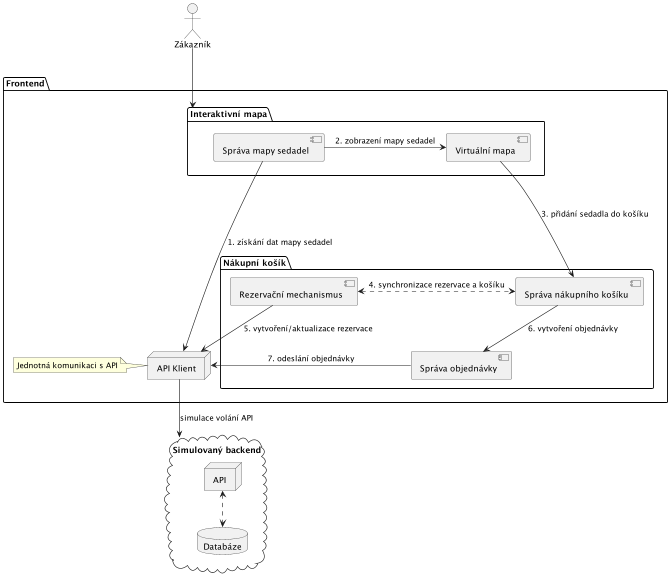
\includegraphics[width=\textwidth]{\FIGDIR/diagrams/architecture}
        \source{}
        \label{fig:implementace-architektura-high-level}
    \end{figure}

    Aplikace se skládá ze tří primárních oblastí, a to interaktivní mapy, nákupního košíku a \ac{api} klienta.

    \textbf{Interaktivní mapa} slouží jako ústřední bod aplikace a poskytuje vizuální znázornění uspořádání sedadel.
    Tato oblast zahrnuje správu mapy sedadel, kde se zpracovávají data získaná z \ac{api}, a také virtuální mapu, která vizuálně prezentuje rozvržení sedadel a umožňuje uživatelům vybrat si požadovaná sedadla.
    Po výběru sedadla systém naváže komunikaci s modulem košíku pro přidání vstupenky se zvoleným sedadlem do nákupního košíku zákazníka.

    \textbf{Nákupní košík} je komplexní prostředí se třemi odlišnými sekcemi.
    \textit{Správa košíku} zahrnuje prezentaci a manipulaci s obsahem košíku, včetně informací o výběru sedadla získaných z virtuální mapy.
    Po kontrole obsahu košíku mají zákazníci možnost vytvořit svou objednávku prostřednictvím \textit{správy objednávek}.
    \textit{Rezervační modul} zajišťuje vytvoření či úpravu rezervace a její harmonizaci s obsahem košíku.

    \textbf{\ac{api} klient} slouží jako univerzální komunikační bod mezi frontendovou aplikací a potenciálním backendem, který by mohl být v budoucnu implementován.
    Zodpovídá za získávání dat mapy sedadel, správu rezervací či vytvoření objednávky.
    Díky tomu, že \ac{api} klient poskytuje pouze jednotné rozhraní pro komunikaci s backendem, je možné v budoucnu snadno implementovat vlastní \ac{api} klient pro komunikaci s jiným backendem.

    V následujících částech budou implementačně rozebrány jednotlivé klíčové oblasti aplikace jako jsou interaktivní mapa sedadel, správa nákupního košíku, rezervační systém a proces vyřízení objednávky.
\end{subsection}
